\zexternaldocument{inleiding}
\zexternaldocument{analyse}

\chapter{Evaluatie}
Om de impact van de verschillende heuristieken te meten volgt nu een overzicht van de testresultaten.
De heuristieken die te maken hebben met intermachinale afhankelijkheden werden grotendeels getest met behulp van een simulator.
De werking van deze simulator wordt uitgelegd in sectie \ref{sec:simulator}

In de daarop volgende secties wordt voor elke heuristiek eerst nog een kort overzicht gegeven, dan de verwachte resultaten en uiteindelijk welke winst er uiteindelijk echt behaald werd.
De algemene verwachting is dat het gebruiken van de heuristieken het aantal deployment runs verkleint en zo ook de totale uitroltijd.
Deze optimalisatie kost wel extra verwerkingstijd (de uitvoering van de verschillende heuristieken) maar deze is normaal gezien te verwaarlozen ten
opzichte van het volledige uitrolproces. 

\section{Simulator}
\label{sec:simulator}

Hoe groter het model wordt, hoe langer het duurt om alles volledig uitgerold te krijgen. 
Zelfs met het gebruik van heuristieken om het aantal deployment runs te minimaliseren blijft een significant deel van het proces gespendeerd aan bijvoorbeeld het downloaden van packages. 
Nog een reden om een simulator te ontwikkelen is dat deze ons toelaat modellen met honderden machines uit te rollen op \'e\'en enkele pc.

De simulator bootst een systeem na dat Fedora 18 draait en gebruik maakt van de yum package manager.

\subsection{Uitwerking}
\label{simulator:uitwerking}
Aan IMP kan gevraagd worden om in plaats van het model uit te rollen, het model op te slaan in JSON formaat.
De simulator gebruikt dat bestand als invoer om het uitrolproces te simuleren.
Het resultaat van een simulatierun is een sqlite-database waarin alle hosts en hun resources vermeld staan.
Om de simulatie zo waarheidsgetrouw mogelijk te maken houdt de simulator rekening met volgende aspecten van het uitrolproces:

\begin{itemize}
  \item Bestanden en mappen kunnen niet aangemaakt worden voordat hun oudermap bestaat
  \item Services kunnen niet gestart worden voordat het bijhorende package en bestanden aanwezig zijn
  \item Resources worden pas aangemaakt als hun afhankelijkheden voldaan zijn
\end{itemize}

De simulator maakt gebruik van twee externe informatiebronnen: een lijst van standaardmappen die aanwezig zijn na een nieuwe Fedora installatie en de repository data van verschillende yum repositories.
Beide helpen bij het nakijken van de voorwaarden voor het aanmaken van respectievelijk bestanden of mappen en services:
voordat een bestand weggeschreven wordt naar de database wordt gekeken of ofwel de parent folder al in de database staat, of dat het een standaardmap binnen Fedora is.
Voor een service wordt in de repositorydata opgezocht welke bestanden normaal gezien deel zijn van de het pakket dat die service installeert en nagekeken of deze aanwezig zijn in de database.
Om deze laatste check te kunnen doen worden bij het wegschrijven van een package ook alle bijhorende bestanden in de database opgeslagen.

De simulator gebruikt hetzelfde beslissingsproces om de uitrolvolgorde te bepalen als IMP.
Dit valt het makkelijkst te beschrijven in pseudocode:

\begin{lstlisting}
%finished_deploying == True als er geen enkele agent nog resources moet deployen
while not finished_deploying:
    for agent in agents:
        no_reqs = [write_to_database(res) for res in agent.resources if not res['requires']]
        for agent in agents:
          for res in agent.resources:
              res.requires.remove(no_reqs)
\end{lstlisting}

%big project deploy met sim
%real   3m36.324s
%user    1m24.040s
%sys 0m23.338s

\section{Afhankelijkheden tussen bestanden en mappen}
\label{sec:bestanden_en_mappen_eval}
Aangezien een bestand niet kan gecre\"eerd worden zonder zijn parent folder voegt deze heuristiek automatisch de afhankelijkheid tussen beide toe aan het model.

Om het effect van deze heuristiek te meten werden verschillende deployment runs gestart met en zonder gebruik van het algoritme.
Sowieso zijn er altijd maar maximaal twee deployment runs nodig als geen heuristiek gebruikt wordt aangezien mappen altijd kunnen gecre\"eerd worden.
De verwachting is dat het uitrollen met gebruik van de heuristiek dan ook ongeveer half zo lang duurt.

Het resultaat van deze testen is te vinden in figuur \ref{fig:file_dir_times}.
Elk datapunt is het gemiddelde van 30 runs, uitgevoerd op een virtuele machine met 2 cores van 2 Ghz en 2 GB RAM ter beschikking.

\begin{figure}[h]
    \begin{center}
    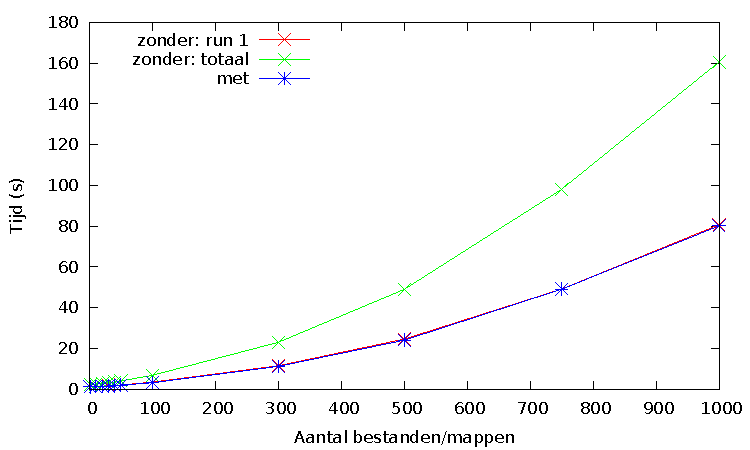
\includegraphics[width=0.8\textwidth]{images/file_dir_times.pdf}
    \caption{Testresultaten bij het uitrollen van een stijgend aantal bestanden en mappen, met en zonder gebruik van de heuristiek}
    \label{fig:file_dir_times}
    \end{center}
\end{figure}

De verwachtingen zijn volledig ingelost: zonder heuristiek zijn er twee deployment runs nodig dus is er dubbel zoveel tijd nodig.

\section{Afhankelijkheden tussen services, packages en configuratiebestanden}
\label{sec:srv_pkg_cfg_eval}
De specificatie van een service in het configuratiemodel gaat vaak gepaard met de package en de configuratiebestanden die die service nodig heeft.
Aangezien de service niet correct werkt zonder de aanwezigheid van de package en de bestanden voegt deze heuristiek de gepaste afhankelijkheden toe aan het model.

Om deze heuristieken te testen werd 30 keer NTP uitgerold op een testmachine.
NTP bestaat uit \'e\'en package, \'e\'en configuratiebestand en \'e\'en service. 
In het slechtste geval zijn er normaalgezien dus drie deployment runs nodig om de service correct werkende te krijgen.
Als de correcte afhankelijkheden worden opgesteld is er slechts \'e\'en run nodig.
De testresultaten zijn te vinden in tabel \ref{table:service_package_dep}.

\begin{table}
  \begin{center}
  \label{table:service_package_dep}
  \begin{tabular}{ r | c | c }
            & tijd(s)   & gemiddeld aantal runs nodig \\ \hline
    zonder  & 3.21      & 2.0 \\ \hline
    met     & 2.21      & 1 \\
  \end{tabular}
  \caption{Meetresultaten}
  \end{center}
\end{table}
%specifieke resultaten:
%zonder
%Avg time: 3.212880388398965
%Deployments avg: 2.0
%met: Avg time: 2.2067235755423704
%deps toegevoegd: 3


De verwachtingen worden weeral ingelost: dankzij de heuristiek is maar \'e\'en deployment run meer nodig.
Dit resulteert niet in een halvering van de uitroltijd aangezien er altijd constante tijd gespendeerd wordt aan de initialisatie van IMP zelf.

\section{Relaties en afhankelijkheden tussen hoog-niveau concepten}

IMP laat toe om basisresources die logisch bij elkaar horen en hergebruikt kunnen worden te groeperen in een concept.
Tussen deze concepten kunnen relaties gespecifi\"eerd worden.
Stel het voorbeeld met een webserver en een databaseserver als concepten.
De relatie tussen beide is als volgt:
\begin{lstlisting}
webserver [0:n] -- [1:n] databaseserver.
\end{lstlisting}
Hieruit leiden we af dat elke webserver altijd een database nodig heeft, maar niet omgekeerd.
Deze afleiding geldt voor alle relaties met gelijkaardige multipliciteiten.

Zoals vermeld in sectie \ref{sec:hoog_niveau_relaties} zorgt deze heuristiek niet zozeer voor een foutloos dan wel een effici\"enter uitrolproces.
Om die reden \todo{aanvullen} 
%No reqs: [10 runs]
%Avg time: 276.6101951248
%32428 Deployments avg: 3.0
%
%No reqs + use_rel_multiplicity en use_relations:
%Stacks found: 392
%Added 72 new dependencies
%292 total dependencies, 645 new requirements added.(vooral depends on firewalld, flens)

%Avg time: 203.78462052040013
%Deployments avg: 2.0

\section{Use cases}

\subsection{Document processing}

\todo{Uitleg geven over usecase}

In afbeelding \ref{fig:reqs} is te zien hoeveel requirements elke heuristiek toevoegen.
De heuristiek die de parent folder toevoegt aan de requirements van een map of bestand wordt altijd uitgevoerd.
Deze heuristiek beschouwen we namelijk als fundamenteel: de requirements die ze toevoegd zijn sowieso juist, terwijl de requirements die door andere heuristieken worden toegevoegd soms overbodig zijn. 

We verwachten dat sommige heuristieken zullen overlappen, bijvoorbeeld ``stack'' en ``name''. 
Resources binnen dezelfde stack hebben namelijk vaak een gelijkaardige naam. 

\begin{figure}[h]
    \begin{center}
    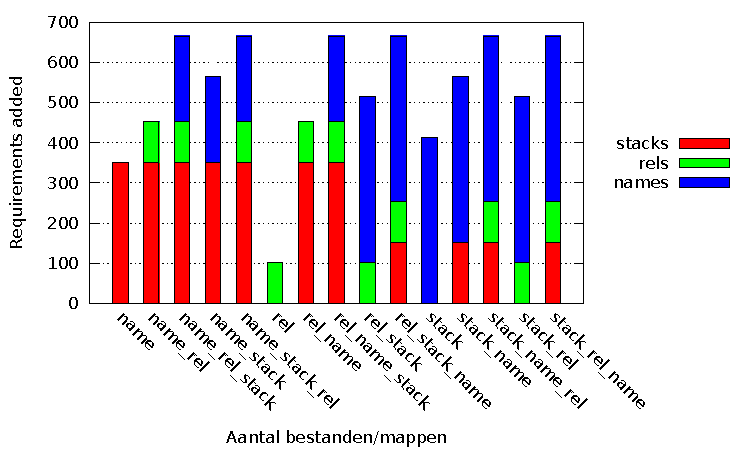
\includegraphics[width=0.8\textwidth]{images/reqs.pdf}
    \caption{Aantal toegevoegde requirements voor elke combinatie van heuristieken}
    \label{fig:reqs}
    \end{center}
\end{figure}

We zien inderdaad dat de heuristieken overlappen.
Als een bepaalde heuristiek eerst toegepast wordt kan hij al zijn requirements toevoegen.
Daaropvolgende heuristieken zullen enkel het deel van hun requirements toevoegen die nog niet deel uitmaken van het model.
Ongeacht de volgorde zal een combinatie heuristieken altijd dezelfde set requirements toevoegen.

In afbeelding \ref{fig:time_runs} is te zien welke impact de toegevoegde requirements hebben op het uitrolproces.

\begin{figure}[h]
    \begin{center}
    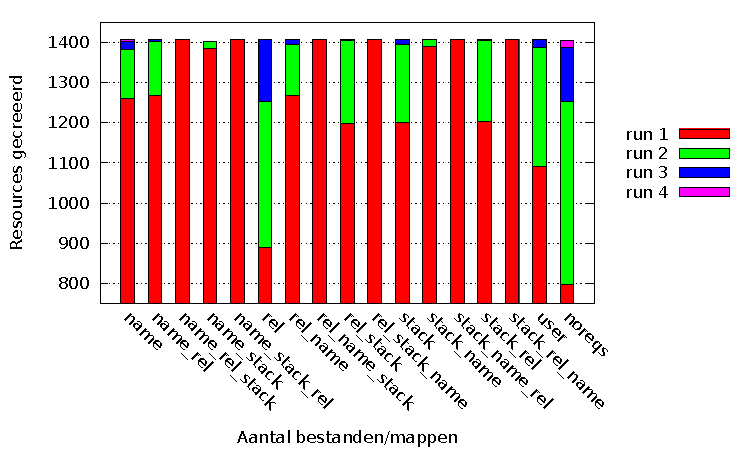
\includegraphics[width=0.8\textwidth]{images/time_runs.pdf}
    \caption{Gemiddelde uitroltijd en aantal deployment runs nodig voor elke combinate van heuristieken}
    \label{fig:time_runs}
    \end{center}
\end{figure}

De resultaten bevestigen onze aanname dat het toevoegen van requirements kan leiden tot een daling in het aantal deployment runs.
Elke combinatie van de drie heuristieken leidt zelfs tot een ``one-shot'' uitrolproces waarin in \'e\'en keer het volledige model correct uitgerold wordt.
\subsection{MongoDB}
